\renewcommand{\thechapter}{6}
\chapter{The Lightmap}
\label{ch:Lightmap}

\textcolor{red}{Explain why the old lightmap was easier to construct [due to the larger signals]}

The EXO-200 detector has roughly 450 APDs ganged into 74 data channels of six or seven APDs each. Three of the APD ganged channels were disabled due to noisy components before physics data collection began; a fourth channel was disabled in February 2012 due to increasing noise.  The APDs are set into the two endcaps of the cylindrical EXO-200 detector.  To improve light collection, teflon sheets cover the inside of the detector and reflect light back into the liquid xenon rather than allowing it to be absorbed by the vessel walls.

Given the same amount of energy deposited into the detector, APDs channels nearest to the deposited energy show significantly larger signals than APD channels far from the deposit.   To accurately measure the true scintillation energy, it is critical to map out the response of the APDs as a function of deposit position $\vec{x}$.

Furthermore, the APDs and their front-end electronics show time-dependent changes. Gains drift in each APD channel at a variety rates, and stepwise changes occur when the electronics are changed or channels are disabled. This has happened on multiple occassions during the course of the experiment.  This means that, in addition to mapping the response of the APDs as a function of deposit position $\vec{x}$, we must also map it as a function of  time. We call this the lightmap.

Earlier lightmaps were derived from periodic source calibration campaigns collected over one or more days. The "strong" Thorium-228 source was used, and an on-site expert would  position the source in a wide range of locations around the detector.  The $2615$-keV single-site gamma line of the Thallium-208 (a daughter product of Thorium-228)allows the signal magnitude from a single-position mono-energetic deposit in the detector to be determined in offline analysis.

Even with such a significant quantity of source data, statistics are generally insufficient to fully characterize the lightmap with this method.  Some regions of the detector are difficult to illuminate with the 2615 keV gamma line, and signals on individual channels are small.  To simplify the problem, signals on each endcap can be summed together (without gain corrections) such that the 70 or 71 active APD channels can be treated as merely two APD channels.  This effectively increases the size of the signals and the signal-to noise. It also makes the spatial dependence of the response smoother, so that a sparser distribution of data is sufficient to characterize the response.  This permitted the creation of an APD-plane lightmap which allowed EXO to produce its first position-dependent corrections to scintillation energy~\cite{ThesisSteve}.

Although this lightmap produced significant improvements in the energy resolution achieved by the EXO detector,  it is an incomplete characterization of the APD response.  For example, for $\beta\beta0\nu$ studies we place a fiducial volume cut as close to the edges of the detector as possible, and in certain regions of the detector the scintillation signal is highly concentrated on a small number of channels.  Summing together multiple channels is, in this case, a lossy form of compression of the data, and it is possible to extract a better energy measurement if it is avoided.  

The denoising algorithm described in chapter~\ref{ch:DenoisingTheory} describes one such method by which we can exploit knowledge of the behavior of individual APD channels; others include reducing our scintillation thresholds by allowing us to search for signals in subsets of the APDs rather than only in sums across entire endcaps.  Thus, characterizing the APD yield on individual APD-gang channels is not in itself an important component of our analysis, but may be expected to provide a critical tool for more advanced scintillation analysis.

\section{Four-Dimensional Lightmap}

As described above, in constructing a channel-by-channel lightmap we face two conflicting needs: we must use as much data as possible to handle the rapid spatial variation and smaller signals which are expected, but if too much data is included then we run the risk of combining data taken when an APD or the electronics had a different gain.  If we truly wish to use all available data, then we must simultaneously understand the full time-dependence of the gain.  In other words, rather than forming a small number of independently-measured three-dimensional lightmaps, we instead measure a four-dimensional lightmap $L(\vec{x},t)$.  Since we use Thorium-228 source data to generate the lightmap, we require that our lightmap should predict the magnitude of the signals on each APD gang induced by a single-site deposit of energy $2615$ keV.  Figure~\ref{fig:SampleAPDTemplates} shows our definition of a unit-magnitude signal.

This may at first seem infeasible.  After all, adding an extra time dimension to the arguments of the lightmap is equivalent to generating a new lightmap for every time bin, which is exactly the situation we wish to avoid.  But we can make a simplifying assumption that the lightmap is separable.  In a physical sense, we assume that:
\begin{enumerate}
\item From a given position $\vec{x}$, photons deposit on each APD channel at a constant rate.
\item Each APD channel amplifies and shapes its signal with a gain which may vary in time, but does not depend on the point of origin of the photons.
\end{enumerate}
So, we demand that the lightmap have the much simpler form
\begin{equation} \label{eqn:SeparableLightmap}
L(\vec{x},t) = R(\vec{x})S(t)
\end{equation}

Although this is a reasonable approximation, there are details which are omited by this model.  Since the electric field and the reflectivity of detector surfaces are constant in time, assumption 1 is likely to be valid.

However, assumption 2 may not hold in certain cases. For example, each channel draws its signal from multiple APDs, each of which has an independent time-varying gain.  Photons from a deposit may preferentially sample the gain from the closest APD within a channel, so deposits in different locations may track more closely the gain of the closest APD within a channel.  A study of the impact of this effect is a topic for future study. The analysis presented here will treat it as a small effect.

One simple scheme to find $R$ and $S$ iteratively is described in algorithm~\ref{alg:LightmapScheme}.  Step~\ref{algline:LightmapFormListOfHits} of that algorithm is to select $2615$-keV single-site events; it is understood that some compton-scattered events will inevitably leak into our selection window, but we use the best available energy measurements to minimize that likelihood. As analysis improvements continue to improve the energy resolution, the number of selected compton-scattered events will become smaller and the quality of the lightmap will improve.  The rest of the algorithm describes how we can efficiently converge on estimates of $R(\vec{x})$ and $S(t)$ through an iterative approach.  We do not prove that the algorithm is guaranteed to converge; however, in practice $S(t)$ is almost constant, resulting in fairly rapid convergence.

\begin{algorithm}
\caption{Generating a Lightmap}
\label{alg:LightmapScheme}
\algsetup{indent=2em} % Recommended by the package authors; the default is only for backward compatibility.
\begin{algorithmic}[1]
\STATE Tabulate, using the best energy measurement available, a list of single-site 2615-keV events from Thorium-228 source data. \label{algline:LightmapFormListOfHits}
\STATE Set $S(t) = 1$ for all APD channels.
\REPEAT
  \STATE For each APD channel, estimate $R(\vec{x}) = L(\vec{x},t)/S(t)$ from the set of events tabulated in line ~\ref{algline:LightmapFormListOfHits}.
  \STATE For each APD channel, estimate $S(t) = L(\vec{x},t)/R(\vec{x})$ from the set of events tabulated in line ~\ref{algline:LightmapFormListOfHits}.
\UNTIL convergence is reached.
\end{algorithmic}
\end{algorithm}


\section{Algorithm Details}

The previous section outlines a general algorithm for computing a four-dimensional channel-by-channel lightmap from source data.  In this section we specify the implementation choices which are made in the code currently in use by EXO-200.  In attempt to encourage future experimentation, alternative options will also be listed in some detail, along with some motivations for these alternatives.  Time has not permitted testing of all of these options, but it is hoped that they will be explored in the future.

\subsection{Event Selection}\label{sec:LightmapEventSelection}

The single-site Thorium-228 spectrum is well-peaked at 2615 keV, making it an excellent monoenergetic calibration line.  Our challenge is to select truly 2615-keV events as efficiently as possible, while simultaneously avoiding near-2615-keV events which may leak into the dataset.

This is inherently an iterative process.  The first lightmap is constructed from events selected based on an ionization-only spectrum because no useful position-corrected scintillation measurement yet exists. The resolution of the ionization-only spectrum is relatively poor, roughly $3.5\%$ (sigma) of the energy, as described in Steve Herrin's thesis, and compromises are made to keep the Compton-shoulder leakage to acceptable levels.  That work required events to have ionization between $0.33\sigma$ and $3\sigma$ of the ionization peak~\cite{ThesisSteve}.

Such a strongly asymmetric cut is chosen to avoid leakage from compton shoulder events.  However, because of the anticorrelation between scintillation and ionization, events whose ionization fluctuates high preferrentially selects events whose scintillation fluctuates low, introducing a bias in the signal magnitude.  Additionally, the cut accepts less than $37\%$ of good events, which is a substantial loss of event statistics. This has a significant impact in certain low-statistics regions of the detector.

The current work benefits from this existing position-corrected scintillation measurement, leading to a rotated energy spectrum with resolution of roughly $1.8\%$.  As a result, it is possible to accept more events while still keeping Compton shoulder leakage small.  We currently accept events within $2\sigma$ of the peak, with better than $95\%$ acceptance and only small leakage.  An additional benefit is that the improved energy resolution allows us to use a symmetric acceptance region, avoiding the implicit bias introduced from the earlier asymmetric cut window.

Preliminary investigations have been conducted to see the impact of using the denoised scintillation measurements which are the subject of this work in the event selection itself.  Presently the improvement in resolution \textcolor{red}{(to roughly $1.4\%$) UPDATE WITH REAL NUMBER when the paper is finalized} has not demonstrated any significant improvement in the quality of the lightmap beyond what we can achieve with $1.8\%$ resolution. This is a topic of continuing study.

Beyond the cuts described above (single-site within an appropriate energy window), other basic cuts are applied to ensure only well-behaved scintillation signals are selected:
\begin{itemize}
\item Charge and light must individually lie within a reasonable range.
\item The charge-to-light ratio must not identify an event as an alpha decay.
\item The scintillation time must be well-separated from any other scintillation signals in same event frame.
\item All charge signals which are assigned to this scintillation signal must be assigned unambiguously.
\item All three position coordinates of the charge deposit must be known.  (No fiducial cut is placed, since that would restrict the volume where the lightmap is specified.)
\end{itemize}
Many of these cuts are probably unnecessary. As the energy resolution has improved, the chances of compton-shoulder contamination have decreased. Note that our analysis only accepts events with a single scintillation signal, a requirement which would carry a high cost in lost statistics for determination of the lightmap.  (Strong Thorium runs produce a significant rate of events with multiple scintillation signals.  These statistics are quite valuable, particularly because they are the primary source of events in some poorly illuminated regions of the detector.)  

\subsection{Function Parametrization} \label{sec:LightmapFunctionParametrization}

Because we are attempting to empirically measure the functions $R(\vec{x})$ and $S(t)$ from a finite dataset, we must specify some more limited form for them to take.  All current approaches to describing $R(\vec{x})$ first bin the detector volume into three-dimensional voxels, and then define $R(\vec{x})$ to interpolate linearly between known values at the center of the voxels.  The size of these voxels must be chosen with some care; if they are too small, then low per-voxel statistics cause the statistical errors on the signal magnitude to dominate, whereas if the voxels are too large then the spatial variation of the lightmap is not fully captured.

In the current lightmap, the detector is binned into $1 cm^3$ voxels; the detector is easily contained within a box with sides $40 cm$ long, leading to $64,000$ voxels (of which roughly $20\%$ lie outside of the detector and will be empty).  The choice of voxel size was made based on the size of an individual APD, which is roughly $2.5 cm$ in diameter. Very near the anode we would like for the size of a voxel to be much smaller than $2.5 cm$.  When this is done, much of the detector has sufficient statistics per voxel; however, there are some regions of the detector with fewer than ten hits per voxel, indicating that $R(\vec{x})$ may have quite significant statistical error in these regions.

It is possible to justify a choice of larger voxels.  The APDs lie at $\pm 204 mm$ from the cathode, which means that there is more than $2 cm$ between our fiducial volume and the APDs.  At this distance, the dependence of the lightmap on $x$ and $y$ is expected to be much slower than at the APD plane, indicating that perhaps $2 cm$ binning in $x$ and $y$ may be sufficient.  Additionally, $z$-dependence of the lightmap is expected to be fairly smooth throughout the detector. Since we interpolate linearly between voxels, it may be possible to use a $z$-binning much coarser than $1 cm$.  This is a topic for future investigation.

It is also worth mentioning that alternative voxel geometries have been tried in the past.  The older APD-plane lightmap~\cite{ThesisSteve} used a cylindrical-coordinate binning. Binning in $r$ was selected to make the bin volumes roughly constant along the $r$ axis, binning in the angular coordinate was uniform, and binning in $z$ was chosen to be coarser near the anodes and finer near the cathode to reflect faster variation there.  In all cases the binning was coarser than with the current cubic voxels being used. Our finer binning is made possible by the larger quantity of available statistics from using the full dataset, and is justified by the potential for the yield on a single APD gang to vary more rapidly than the yield averaged across an entire APD plane.

It is well-known~\cite{MultivariateDensityScott} that when it is necessary to estimate a multivariate function from limited statistics, a choice of binning can have a significant impact on the result.  It is preferable to use an unbinned technique such as kernel regression.  In particular, our data density is highly non-uniform, and it should be possible to measure the lightmap with high fidelity in regions of high statistics, while smoothly transitioning to a coarser interpolation in regions of low statistics to minimize the impact of uncertainty from individual hits.  State-of-the-art solutions to this problem would rely on locally adaptive kernel regression; see~\cite{MultivariateDensityScott} for a detailed explanation of the related issues in non-parametric multivariate regression.  Attempting to use a locally adaptive kernel regression for $R(\vec{x})$ should be considered a highly appealing extension to the algorithm described here for generating a lightmap.

The parametrization of $S(t)$ presents a very different set of choices.  Thorium data is taken in bursts, with the time between mostly filled by low-background runtime.  When we choose to treat $S(t)$ as a smoothly varying function, it becomes critical to interpolate properly -- after all, the low-background runtime is the critical part of the experiment.  (If we only produce a lightmap accurate during source calibration runtime, we will measure an energy resolution from source data which is not borne out in the low-background data, so we should in fact be able to give some guarantee that $S(t)$ is almost as accurate during the low-background runtime as during the source runtime.)  Fortunately, it is generally true that the time variation of the APD response is quite slow; exceptions are generally due to changes in the electronics which occur at well-specified times.

Currently each source run is treated as a burst of data taken at the midpoint of the run, and $S(t)$ is measured at that point only from the data of that run; then $S(t)$ is linearly interpolated between those points.  In principle it is possible that between two source runs an electronics change may have been performed, which would mean that a better interpolation would be to assume $S(t)$ is flat except for a step at the time of the electronics change; in practice, though, EXO-200 has generally taken a source run immediately before and after an electronics change, so no high-value data is taken during that interval and this detail can be ignored.

Another concern with this method is the treatment of short source runs.  If a run is too short, then the measurement of $S(t)$ coming from that run may have significant errors.  We currently mitigate this issue by entirely throwing out all data from runs with fewer than $100$ usable events.  We justify this approach by claiming that even though those events might in principle have contributed some useful information on $R(\vec{x})$, without a good measurement of the relevant $S(t)$ it is impossible to use that data.

In the future, it would be useful if instead we performed smoothed interpolations between electronics changes.  This could be done in the same style as EXO's lifetime corrections, using polynomial fits, where the degree of the polynomial could be determined by eye.  A candidate set of time intervals when $S(t)$ might be treated as constant could be the same as the set of constant noise windows described in chapter~\ref{ch:NoiseMeasurements}.  It would be possible to check whether this time binning is fine enough by looking at the Thorium scintillation peak position versus time in denoised data -- if it appears to drift in time within a window where $S(t)$ is treated as constant, then it is likely that $S(t)$ needs to be binned more finely.

Alternatively, often there is a long string of consecutive source runs which should be combined into one higher-statistics dataset.  This process must be done by hand, and has not been performed for the current analysis, but it could benefit the accuracy of the $S(t)$ function and also recover some statistics in cases where the individual runs might be too short for inclusion in the lightmap dataset.

The choice of binning or parametrization for $R(\vec{x})$ and $S(t)$ can have a profound impact on the accuracy of the lightmap, and the current analysis has only skimmed the surface of the various options.  It is hoped that further work on the lightmap will include significant investigation in these topics.

\subsection{Convergence and Error Estimation}

Our treatment of the convergence of algorithm~\ref{alg:LightmapScheme} and the resulting statistical errors in $L(\vec{x}, t)$ is rudimentary.  Cronvergence is checked not by analysis of the lightmap itself, but by verifying that the energy resolution from denoising is not improved by further iterations through algorithm~\ref{alg:LightmapScheme}.  Lightmap errors do not directly enter into the calculations of denoising (which treats the lightmap as perfectly known), so they are not estimated at all in the current analysis.

As a proxy for estimation of the statistical errors in the lightmap, we instead study the number of hits observed in each position voxel of the detector (see section ~\ref{sec:LightmapVisualization}), and presume that the most significant source of error comes from low-statistics regions of the detector.  This information can motivate future data-taking campaigns to probe the light response in those regions of the detector and reduce these uncertainties.  However, no explicit estimation of the lightmap uncertainty has been attempted.

One difficulty with estimating the errors in the lightmap function $L(\vec{x},t)$ comes from the correlation between errors in $R(\vec{x})$ and $S(t)$.  If one of those two components were known perfectly, then we could treat the fit uncertainties of each hit as independent errors, and propagate those errors into an uncertainty for each voxel of $R(\vec{x})$ (if $S(t)$ is assumed to be perfectly known) or $S(t)$ (if $R(\vec{x})$ is assumed to be perfectly known).  But on the contrary, all of the measurements of $R(\vec{x})$ are correlated with all of the measurements of $S(t)$, meaning that even the errors of different voxels of $R(\vec{x})$ or different times in $S(t)$ are correlated with each other.  Fully characterizing these errors would require a significant effort and computation.

Although a full estimate of lightmap errors with correlations would probably be computationally quite intensive to produce, it might be possible to estimate the independent errors of each voxel of the position lightmap $R(\vec{x})$ or each independent run making up $S(t)$ by treating the other function as perfectly known, as described above.  This would generally produce an underestimate of the uncertainty in each, but the estimate might still give some benefit.

To produce a more accurate estimate of errors, it would probably be necessary to do a simultaneous fit by varying both $R(\vec{x})$ and $S(t)$ together.  In the current scheme, $R(\vec{x})$ contains far more complexity than $S(t)$ with roughly $50,000$ non-empty voxels, so for each APD gang we would need to simultaneously vary roughly $50,000$ parameters to obtain the optimal lightmap.  It is exactly this time-intensive process which was avoided by choosing the iterative approach for measuring the lightmap; however, it would only need to be performed occasionally when deriving a new lightmap, so it is not infeasible to imagine attempting this project.  The prospect of feeding in a high-quality guess obtained from the iterative method presents an additional significant time-saver.  This method would not fully account for the correlations between errors of the different voxels of $R(\vec{x})$ or runs in $S(t)$, but it would come closer than the naive method described earlier.

However, it is also possible that identifying the error of each voxel or run is heading down the wrong path.  As described earlier, it is likely that the optimal (lowest-error) method for estimating the lightmap will be an unbinned method such as a locally-adaptive kernel regression method.  Error estimation in kernel regression presents significant additional challenges compared to errors from binned parametrizations.  At present, I am not aware of any simple scheme to manage this difficulty, meaning that there may be a paradoxical tradeoff that using the best method for minimizing lightmap errors simultaneously makes those errors infeasible to estimate.

Note that under the iterative method, the most naive method for estimating errors is not valid.  It might appear that when $S(t)$ is initialized to a constant value of $1$, we could also assign to it some constant error.  Then when we compute $R(\vec{x})$, we could propagate independent errors from the fit uncertainties of signals and from $S(t)$; and when we compute $S(t)$ we could propagate independent errors from the fit uncertainties and from $R(\vec{x})$; and so forth.  However, such a scheme provides no compensating feedback mechanism to force the iterated errors to a reasonable or accurate value, so there is no reason to believe the errors from such a system (if, that is, they converge at all).  This difficulty may underscore the fundamental challenge associated with measuring the lightmap errors within our scheme -- iterative methods are well-suited to solving a system, but when correlated errors are mistreated as uncorrelated an iterative method can easily magnify the impact of that mistreatment.

On the topic of convergence, it has been mentioned already that by starting with a generally accurate initial guess for $S(t)$ as constant, the iterative solution method tends to converge rapidly.  As a result, and because iterations take only a few hours to perform on a single machine, we currently perform three iterations and claim that convergence is approximately reached.  Ideally, we would require that none of the position voxels or runs change value within an iteration by more than some fraction of their estimated errors; but in the absence of estimated errors, this is of course impossible.

It would be possible, in a conservative approach, to require each value to converge to some small fraction of an ADC unit, ensuring that the convergence is better than our ability to measure signals.  Such a requirement might force us to compute more iterations than are truly warranted by our lightmap errors, but given the reasonable speed of each iteration, such a method still might not be unreasonable.

\section{Implementation for this Analysis}

The physics analysis which will be described in this paper includes data from EXO runs $2464$ to $5597$, which were taken between October 5, 2011 and September 1, 2013.  However, at the time when the initial denoising processing was begun, the tentative range of runs to be used only extended up to $5367$ on June 24, 2013.  As a result, calibrated data at that point was only available up to June 24, 2013, and the lightmap had only been generated using the same set of Thorium source data.

When the run range for the present analysis was extended, a significant portion of the dataset had already been denoised with the lightmap based only on data extending to June 24, 2013.  Although the possibility of creating a new lightmap was considered, this would have required a re-analysis and re-verification of the existing denoised dataset.  As a result, the existing lightmap continued to be used.  The functions $S(t)$, which had only been directly measured up to June 24, 2013, were assumed to remain constant between June 24 and September 1, 2013; no known changes to the APDs occurred during this time, nor did any known environmental factors change, so this assumption was considered acceptable.  Future lightmaps of course will make use of a more complete dataset rather than relying on extrapolation.

Furthermore, one bug was discovered in the lightmap which was used for denoising.  A set of Radium-226 source data was taken before the corresponding identifier could be set in data files, and as a result they were provisionally labeled as Thorium runs.  These runs were mistakenly incorporated into the generated lightmap, and events from the $2204$-keV gamma line of the Bismuth-214 daughter product of Radium-226 were selected and handled as though they were legitimate $2615$-keV events.

It was possible to partially remedy this after the fact: since currently there is a one-to-one relationship between individual source runs and their corresponding points in the functions $S(t)$, it was possible to artificially erase the data points of $S(t)$ originating from Radium runs.  It is not so easy to remove the impact they may have had on $R(\vec{x})$.  However, the Radium runs were taken at a location which is extremely well-populated by Thorium data throughout the life of the detector; since the quantity of Radium data is small by comparison, the effect on $R(\vec{x})$ is presumed to be quite small.  Subsequent studies using a correctly-generated lightmap on small subsets of data indicate that the effect is indeed negligible, as expected.

\section{Visualization} \label{sec:LightmapVisualization}

\begin{figure}
\begin{center}
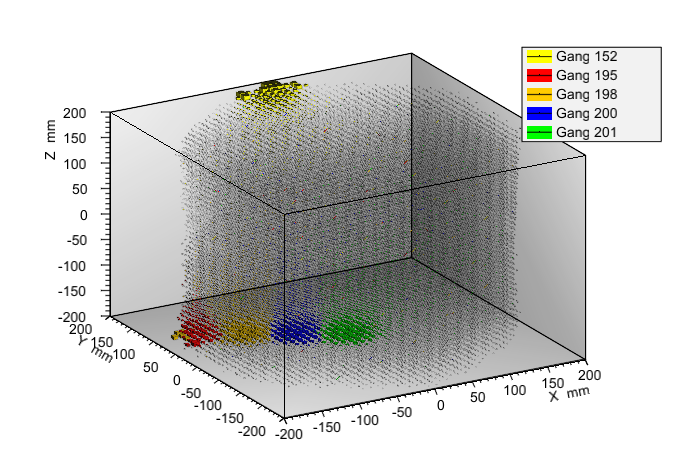
\includegraphics[keepaspectratio=true,width=\textwidth]{Lightmap_viz.png}
\end{center}
\renewcommand{\baselinestretch}{1}
\small\normalsize
\begin{quote}
\caption{Lightmap position-dependence $R(\vec{x})$ for selected APD gangs.}
\label{fig:Lightmap3DPlot_unzoomed}
\end{quote}
\end{figure}
\renewcommand{\baselinestretch}{2}
\small\normalsize

\begin{figure}
\begin{center}
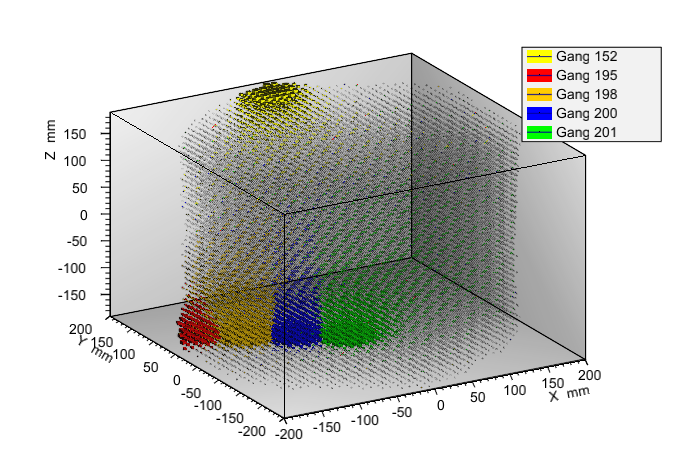
\includegraphics[keepaspectratio=true,width=\textwidth]{Lightmap_viz_zoom.png}
\end{center}
\renewcommand{\baselinestretch}{1}
\small\normalsize
\begin{quote}
\caption{Lightmap position-dependence $R(\vec{x})$ for selected APD gangs.  Here extreme anode positions are omitted to permit better contrast for the lightmap in the fiducial volume.}
\label{fig:Lightmap3DPlot_zoomed}
\end{quote}
\end{figure}
\renewcommand{\baselinestretch}{2}
\small\normalsize

\begin{figure}
\begin{center}
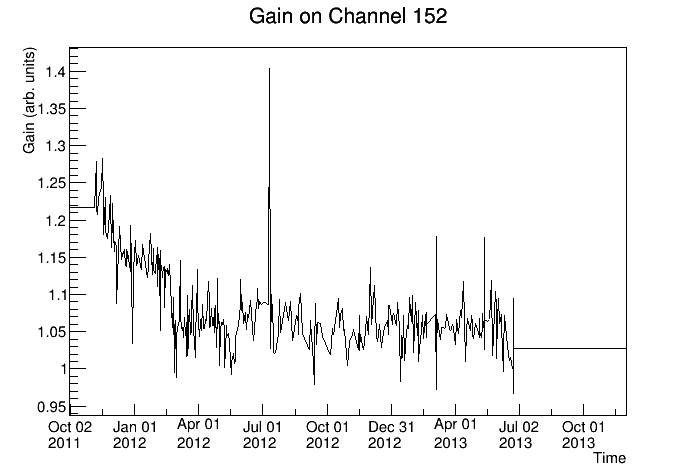
\includegraphics[keepaspectratio=true,width=\textwidth]{gainfunc_152.png}
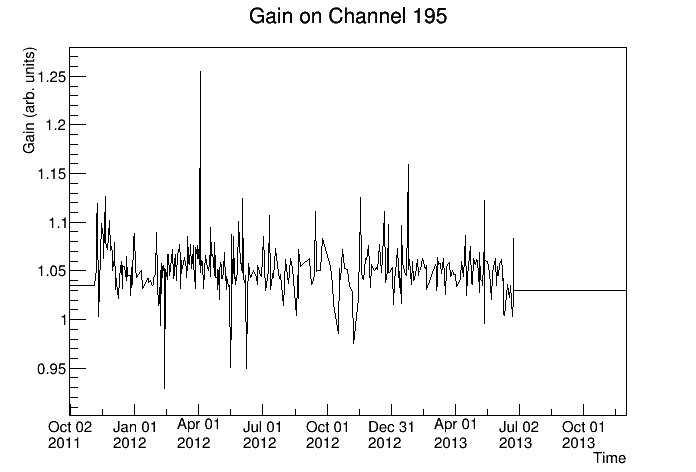
\includegraphics[keepaspectratio=true,width=\textwidth]{gainfunc_195.png}
\end{center}
\renewcommand{\baselinestretch}{1}
\small\normalsize
\begin{quote}
\caption{Functions $S(t)$ for selected channels.}
\label{fig:LightmapGainFunc1}
\end{quote}
\end{figure}
\renewcommand{\baselinestretch}{2}
\small\normalsize

\begin{figure}
\begin{center}
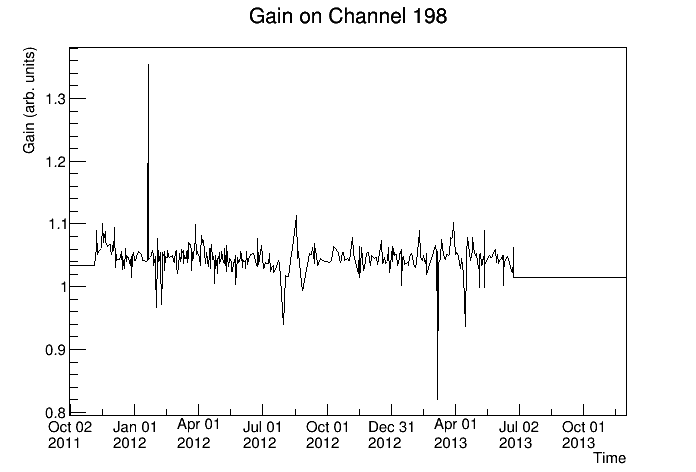
\includegraphics[keepaspectratio=true,width=\textwidth]{gainfunc_198.png}
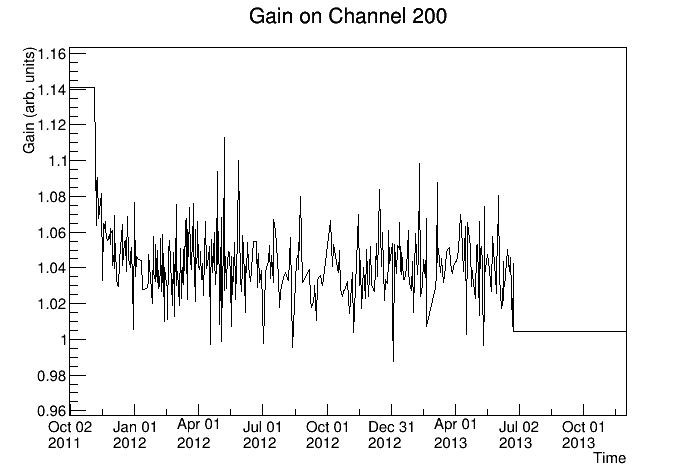
\includegraphics[keepaspectratio=true,width=\textwidth]{gainfunc_200.png}
\end{center}
\renewcommand{\baselinestretch}{1}
\small\normalsize
\begin{quote}
\caption{Functions $S(t)$ for selected channels.}
\label{fig:LightmapGainFunc2}
\end{quote}
\end{figure}
\renewcommand{\baselinestretch}{2}
\small\normalsize

\begin{figure}
\begin{center}
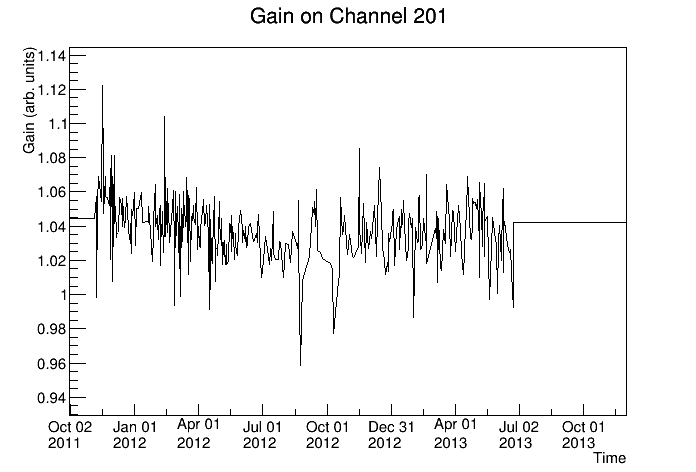
\includegraphics[keepaspectratio=true,width=\textwidth]{gainfunc_201.png}
\end{center}
\renewcommand{\baselinestretch}{1}
\small\normalsize
\begin{quote}
\caption{Functions $S(t)$ for selected channels.}
\label{fig:LightmapGainFunc3}
\end{quote}
\end{figure}
\renewcommand{\baselinestretch}{2}
\small\normalsize

Although it is not strictly necessary to be able to visually inspect the lightmap for it to be useful, nevertheless it is reassuring to see that the lightmap is qualitatively similar to intuitive expectations of how light should propagate through the detector.  We have chosen to store the position-dependent $R(\vec{x})$ for each APD gang as a set of ROOT TH3D objects, and fortunately ROOT provides a number of excellent plotting features suitable for a three-dimensional dataset.  In figure~\ref{fig:Lightmap3DPlot_unzoomed}, it is possible to view the values of $R(\vec{x})$ for a sample of gangs on top of each other.  Larger boxes and denser color indicates a higher yield on the APD gang in question, and it is immediately apparent that events near the anodes produce light which is highly concentrated on a single APD gang.

Figure~\ref{fig:Lightmap3DPlot_unzoomed} shows the highest yield on the very boundary of the detector, well outside of our fiducial volume; to permit us to more easily view contrast inside of the detector, figure~\ref{fig:Lightmap3DPlot_zoomed} shows the same map while omitting the most extreme bin near either anode.  Viewing this map, we can see more interesting characteristics of the lightmap:
\begin{itemize}
\item Events near the anodes show a high signal concentration on the one gang nearest to their position; however, even deep into the detector near the cathode it is still possible to see the higher concentration of signal on the gang directly aligned with the event.
\item We can also see, from gang 201 (green) in this visualization, that events can produce significant signal on APD gangs which which they are not directly aligned (in the Z direction); yield on gang 201 can be seen to decrease smoothly in all directions.
\item APD gangs in the corners of the detector, such as gang 195 (red), are not effective at measuring light from events which are far away; even directly above gang 195, it is clear that gang 198 is more effective at collecting light farther away than about five to ten centimeters.  This can be attributed to the reflection of photons by teflon, which may enhance the light yield on gangs which are not hidden in corners.
\end{itemize}

Figures~\ref{fig:LightmapGainFunc1}, \ref{fig:LightmapGainFunc2}, and~\ref{fig:LightmapGainFunc3} show the functions $S(t)$ for the same sample of gangs.  The vertical scale can be treated as having arbitrary units; we note that all of these functions lie roughly around $1$, which is attributed to the initial placement of $S(t) = 1$ in algorithm~\ref{alg:LightmapScheme}.  We draw the following primary observations from these plots:
\begin{itemize}
\item Many of the gangs show their values of $S(t)$ decreasing rapidly up to around February 2012; some of the gangs also show a sharp decrease in value at that point.  The decrease in gain corresponds with observations which were made at the time, leading to a decision to replace electronics on some APD channels on February 23, 2012.  Thus, we do see ``real" features from these plots.
\item The functions $S(t)$ are otherwise dominated by jitter between points, indicating that we do not collect enough statistics from each run to sufficiently constrain $S(t)$.  This is taken as the strongest evidence that we should use a coarser time binning for $S(t)$, as described in section~\ref{sec:LightmapFunctionParametrization}.  Preliminary work has been performed to do this with more recent lightmaps, but no studies have evaluated the impact on energy resolution.
\item Individual points on these functions may spike by as much as $40\%$.  These points have been investigated, and their cause is not understood.  These jumps, along with the overall jitter, will certainly be reduced by the use of a coarser time binning.
\end{itemize}
